%!TEX root = ../tesis.tex
%!TEX root = ../tesis.tex
\subsection{Modelos Ocultos de Markov}
\label{sec:hmm}

Para introducir el concepto de modelo oculto de Markov (\gls{hmm} por sus siglas en ingl\'es), 
en el cual se basa el proceso de reconocimiento del habla que se busca explicar, 
se utilizar\'a un ejemplo cl\'asico de la literatura relacionada con el tema.
El ejemplo se denomina \emph{El modelo de la urna y la pelota} \cite{Rabiner89atutorial}:

\begin{quote}
	Se asume que hay N urnas (grandes) de vidrio en una habitaci\'on. Dentro de cada urna hay un gran 
	n\'umero de pelotas de colores.
	Un genio est\'a en la habitaci\'on y, de acuerdo a un proceso aleatorio, elige una urna inicial. 
	De esta urna extrae una pelota de manera aleatoria y su color se anota como la observaci\'on, 
	pues el observador desconoce la urna de donde sali\'o la pelota.
	La pelota se coloca de nuevo en la urna y se repiten la selecci\'on de la urna y la pelota respectivamente.
	Este proceso genera una secuencia aleatoria de colores.
\end{quote}

En el caso mencionado, puden distinguirse dos procesos estoc\'asticos:
\begin{itemize}
	\item Del primer proceso se obtiene como salida una secuencia de urnas. Sin embargo, el observador
	no puede visualizar esta secuencia, es decir, la misma permanece oculta.
	\item Del segundo proceso se obtiene como salida una secuencia de colores. La probabilidad de observar
	un color depende de la urna seleccionada previamente, debido a que la cantidad de pelotas de un determinado
	color var{\'\i}a en cada urna.
\end{itemize}

Este sencillo sistema puede modelarse como un modelo oculto de Markov definiendo los siguientes par\'ametros:
\begin{enumerate}
	\item El n\'umero de urnas, a las cuales se denomina estados del modelo.
	\item La cantidad de colores posibles de las pelotas en las urnas, a los cuales se 
	denomina s{\'\i}mbolos observables.
	\item Una funci\'on que determina la transici\'on entre urnas.
	\item Una funci\'on que determina la elecci\'on de una pelota de determinado color, dada una urna.
	\item Una funci\'on que determina la elecci\'on de la urna inicial.
\end{enumerate}

Con la ayuda de este ejemplo, podemos definir formalmente un \gls{hmm}. Un modelo oculto de Markov es un 
aut\'omata finito estoc\'astico entrenable \cite{KouemouHistory2011}, que implica un doble proceso estoc\'astico:

\begin{itemize}
\item El primer proceso, que produce una secuencia de estados, no es observable. Esto es, la secuencia de estados 
que produce permanece oculta.
\item El segundo proceso produce una secuencia de observaciones, donde la probabilidad de 
una observaci\'on est\'a dada por una funci\'on definida para cada estado correspondiente al primer proceso.
\end{itemize}

Un modelo oculto de Markov puede ser caracterizado mediante los siguientes elementos \cite{Rabiner89atutorial}:

\begin{enumerate}
	\item $N$, el n\'umero de estados del modelo. Se representan los estados individuales como: 
		\begin{align}
			S=\{S_1,S_2,\ldots,S_N\}\label{eq:hmmS}
	\end{align}

	\item $M$, el n\'umero de s{\'\i}mbolos observables por estado. Se representan los s{\'\i}mbolos individuales 
		como: 
		\begin{align}
			V=\{v_1,v_2,\ldots,v_M\}\label{eq:hmmV}
	\end{align}

	\item La distribuci\'on de probabilidad de transici\'on de estados $A = \left\{a_{ij}\right\}$.
		Siendo $q_t$ el estado del modelo generado en el tiempo $t$, puede definirse $a_{ij}$ como:

		\begin{align}
			a_{ij} = P[q_{t+1} = S_j \mid q_t = S_i], & & 1 \leq i,j & \leq N\label{eq:hmmA}
		\end{align}

	\item La distribuci\'on de probabilidad de los s{\'\i}mbolos observables en el estado $j$, $b_j(v_k)$. 
		Esta distribuci\'on es una funci\'on de la observaci\'on $v_k$, definida en cada estado.
		Siendo $q_t$ el estado del modelo generado en el tiempo $t$:

		\begin{align}
			b_j(v_k) = P[v_k \text{ en el momento } t \mid q_t = S_j], & & 1 \leq j & \leq N \label{eq:hmmB}
			\\& & 1 \leq k & \leq M \nonumber
		\end{align}

	\item La distribuci\'on de probabilidad del estado inicial $\pi=\left\{\pi_i\right\}$, donde:
		\begin{align}
			\pi_i = P[q_1=S_i], & & 1 \leq i \leq N \label{eq:hmmPI}
		\end{align}
\end{enumerate}

\begin{figure}[H] 
\centering
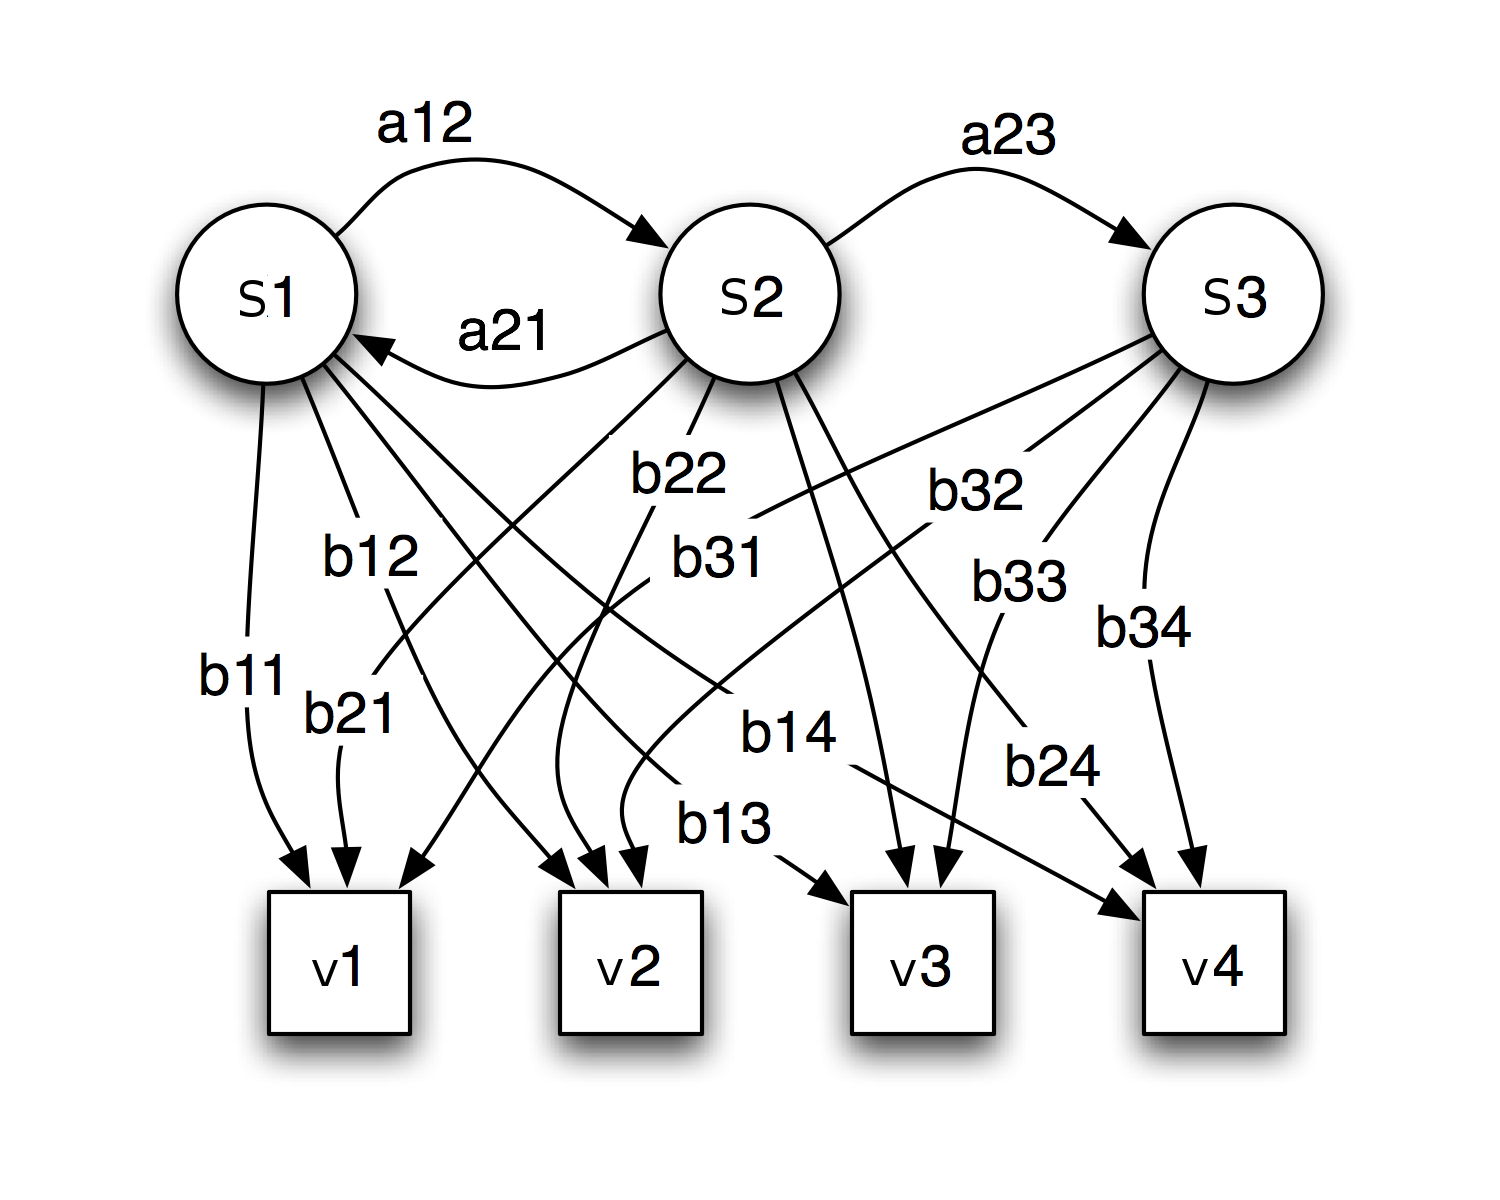
\includegraphics[width=0.8\textwidth]{./graphics/hmm.png}
\caption{Representaci\'on gr\'afica de un modelo oculto de Markov.}
\label{figure:hmm}
\end{figure}

\section[El Reconocimiento del Habla como Problema Estad{\'\i}stico]
{El Reconocimiento del Habla como Problema \\ Estad{\'\i}stico}

Para un lenguaje $L$ y una entrada ac\'ustica $X$, el problema del reconocimiento del habla puede definirse 
como \cite{Jurafsky}:

\begin{quote}
\emph{La b\'usqueda de la oraci\'on m\'as probable perteneciente al lenguaje L, dada la entrada ac\'ustica X.}
\end{quote}

La secuencia de observaciones ac\'usticas $O$ puede representarse como:

\begin{align}
O = o_1,o_2,o_3,\ldots,o_T\label{eq:asrO}
\end{align}

donde la se\~nal de voz fue dividida en $T$ muestras de igual duraci\'on.

La oraci\'on de salida, a su vez, puede representarse como:

\begin{align}
\hat{W}  = w_1,w_2,w_3,\ldots,w_M\label{eq:asrW}
\end{align}

donde la cadena est\'a compuesta por $M$ palabras.

De esta manera, la definici\'on introducida anteriormente puede expresarse matem\'aticamente como:

\begin{align}
\hat{W} = \argmax_{W \in L} P(W|O)
\end{align}

Usando la Regla de Bayes la expresi\'on anterior puede reescribirse como:

\begin{align}
\hat{W} = \argmax_{W \in L} \frac{P(O|W)P(W)}{P(O)}
\end{align}

Como se desea obtener la oraci\'on con mayor probabilidad dada una entrada ac\'ustica, la entrada es
la misma para todas las oraciones evaluadas y su probabilidad de ocurrencia $P(O)$ se mantiene constante.
Puesto de otra manera, el t\'ermino $P(O)$ es independiente de $W$, por lo cual puede despreciarse. 

Por tanto:

\begin{align}
\hat{W} = \argmax_{W \in L} P(O|W)P(W)
\end{align}

El primer t\'ermino representa la probabilidad de una entrada ac\'ustica dada una secuencia de palabras, tambi\'en
conocida como verosimilitud de observaci\'on o modelo ac\'ustico. El segundo t\'ermino es la probabilidad 
\foreign{a priori} de ocurrencia de una secuencia de palabras, tambi\'en conocida como probabilidad previa o 
modelo de lenguaje. Esto es:

\begin{align}
\hat{W} = \argmax_{W \in L} \overbrace{P(O|W)}^\text{M. ac\'ustico}\overbrace{P(W)}^\text{M. de lenguaje}
\label{eq:asrFundamental}
\end{align}

Esta ecuaci\'on es el fundamento del enfoque estad{\'\i}stico al problema del reconocimiento del habla, base de los
sistemas \mbox{modernos \cite{RabinerStatistical2006}}.

\begin{figure}[H] 
\centering
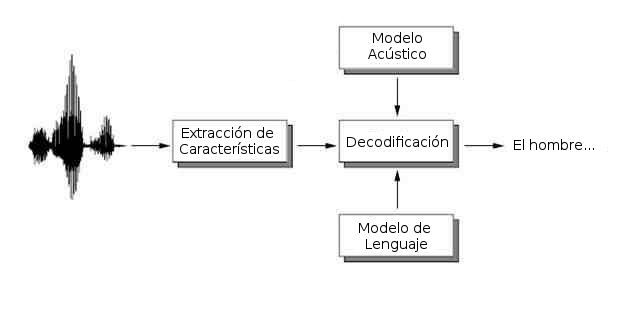
\includegraphics[width=0.8\textwidth]{./graphics/proceso.png}
\caption{Proceso b\'asico del reconocimiento del habla. Traducido a partir de \cite{VerenichASR}.}
\label{figure:proceso}
\end{figure}

La figura \ref{figure:proceso} ilustra de modo general la arquitectura de un sistema de reconocimiento del habla.
El proceso b\'asico del reconocimiento del habla, puede descomponerse en dos etapas o fases, cada una de las cuales
recibe una entrada (o varias) y produce una salida determinada.

%Figura Jurafsky
\begin{itemize}
\item La primera fase o \emph{extracci\'on de caracter{\'\i}sticas} tiene como objetivo caracterizar la se\~nal
de voz para obtener una representaci\'on adecuada para el decodificador. Para tal efecto, produce vectores de
caracter{\'\i}sticas espectrales a partir del sonido que recibe como entrada.
\item La segunda fase o \emph{decodificaci\'on} tiene como objectivo producir la secuencia de palabras m\'as probable
dados los vectores de caracter{\'\i}sticas resultantes de la fase anterior. Para ello se sirve un modelo ac\'ustico, un
modelo de lenguaje y un algoritmo de decodificaci\'on.
\end{itemize}

Las siguientes secciones explican de manera m\'as detallada los conceptos y algoritmos relacionados a cada fase.
Tanto el modelo ac\'ustico como el modelo de lenguaje pueden requerir una fase de entrenamiento, 
previa a la utilizaci\'on del sistema de reconocimiento del habla.
Por motivos de claridad, los detalles de esta fase se presentan en \'ultimo lugar.

%!TEX root = ../tesis.tex
\subsection{Fase 1: Extracci\'on de caracter{\'\i}sticas}
\label{sec:featureExtraction}

En la primera fase, la entrada es la se\~nal de voz correspondiente al emisor, la cual se divide en muestras de corta
duraci\'on llamadas tramas. A trav\'es de un proceso de procesamiento de la onda sonora, se obtienen vectores de 
caracter{\'\i}sticas representativas para cada trama. Esta secci\'on describe los conceptos relacionados a esta 
transformaci\'on.

\subsubsection{Ondas Sonoras}

La entrada para un reconocedor del habla, y en particular para la fase 1, es la misma que la del o{\'\i}do humano: una 
serie de cambios en la presi\'on del aire \cite{YoungUniversity2007}. Estos cambios se originan en el emisor, y son 
causados por el aire que es expulsado de los pulmones, pasa por el tracto vocal y salen por la boca. As{\'\i}, para el 
proceso de s{\'\i}ntesis del habla en el ser humano, los pulmones son la fuente
del sonido y el trato vocal es el filtro que genera los distintos tipos de \mbox{sonido \cite{BradburyLineal2000}}.

Como mencionaba Semat ya en los a\~nos 50, existen dos aspectos del sonido: el f{\'\i}sico y el perceptual. De acuerdo al 
aspecto considerado, var{\'\i}an los t\'erminos con los cuales se describe al sonido; as{\'\i}, un f{\'\i}sico describe un 
sonido en t\'erminos de frecuencia, amplitud y n\'umero de sobretonos, mientras un m\'usico utiliza t\'erminos como tono, 
volumen o \mbox{timbre \cite{SematPhysics1958}}.

Aunque no existe una correspondencia directa entre las car\'acter{\'\i}sticas f{\'\i}sicas y las perceptuales 
\cite{SematPhysics1958}, existe una correlaci\'on en ciertos casos. As{\'\i}, para los sonidos con una frecuencia alta se 
percibe un tono m\'as agudo, aunque esta relaci\'on no es lineal. Igualmente, a mayor amplitud de una onda sonora esta se 
percibe con mayor \mbox{volumen \cite{YoungUniversity2007}}.

\subsubsection{Espectro}
El an\'alisis espectral est\'a basado en la conclusi\'on de Fourier que establece que una onda compleja puede ser 
representada como la sumatoria de varias ondas simples a diferentes frecuencias. El espectro es la representaci\'on de las 
distintas frecuencias que componen una onda, que puede visualizarse mediante una gr\'afica de amplitud en funci\'on de la 
\mbox{frecuencia \cite{Jurafsky}}. 

Los picos espectrales del espectro del sonido se conocen como formantes \cite{Fant1960acoustic}. Distinto fonemas poseen 
formantes a frecuencias determinadas, raz\'on por la cual el an\'alisis espectral tiene un rol determinante en la 
determinaci\'on de la identidad de vocales y otros \mbox{fonemas \cite{LadefogedCourse2006}}.

%Figura%

Un espectrograma, por su parte, es una matriz de celdas indexadas por frecuencia en el eje vertical y por tiempo en el eje 
horizontal, donde el nivel de sombreado de una celda indica la amplitud de la componente a una frecuencia y un tiempo 
dados. Aunque rara vez se use directamente para caracterizar la se\~nal, por resultar poco conveniente en t\'erminos del 
tama\~no de la representaci\'on, la gran mayor{\'\i}a de las caracter{\'\i}sticas utilizadas para el reconocimiento del 
habla est\'an basadas en el \mbox{espectrograma \cite{Ellis08anintroduction}}.

%Figura%

\subsubsection{Proceso de Extracci\'on de Caracter{\'\i}sticas}
El proceso puede resumirse en los siguientes pasos \cite{Jurafsky}:

\begin{enumerate}
\item \emph{Muestreo}: consiste en medir la amplitud de la se\~nal en un momento dado; la frecuencia de muestreo es el 
n\'umero de muestras que se toma por segundo. 

De acuerdo a la f\'ormula de Nyquist, es necesario que la frecuencia de muestreo sea al menos el doble de la frecuencia 
correspondiente a la onda que se desea medir. Por ejemplo, para las conversaciones telef\'onicas, cuyas frecuencias no 
superan los 4000 Hz, una frecuencia de muestreo de 8000 Hz resulta suficiente.

\item \emph{Cuantificaci\'on}: consiste en representar el n\'umero real correspondiente a la amplitud como un n\'umero entero, normalmente de 8
o 16 bits, para cada muestra. Con este paso finaliza la transformaci\'on de anal\'ogico a digital de la se\~nal de voz.

\item \emph{Conversi\'on}: una vez digitalizada, la se\~nal se convierte a un conjunto de caracter{\'\i}sticas espectrales. Los detalles de este 
paso dependen en gran medida del conjunto de caracter{\'\i}sticas que se selecciona para representar a la se\~nal.

\end{enumerate}

\subsubsection{Caracter{\'\i}sticas}
Un buen conjunto de caracter{\'\i}sticas re\'une las siguientes cualidades \cite{KesarkarFeature2003}:
\begin{itemize}
\item Las caracter{\'\i}sticas son perceptualmente significativas, es decir, an\'alogas a las utilizadas por el sistema 
auditivo humano.
\item Las caracter{\'\i}sticas son invariantes, es decir, robustas con respecto a las variaciones en el canal y el emisor.
\item Las caracter{\'\i}sticas capturan la din\'amica espectral, es decir, los cambios del espectro en el tiempo.
\end{itemize}

Algunos de los conjuntos de caracter{\'\i}sticas que se utilizan son:
\begin{itemize}
\item \emph{Codificaci\'on Predictiva Lineal (LPC)}: representaci\'on del espectro basada en la idea de que una muestra 
sonora puede ser aproximada mediante la combinaci\'on lineal de muestras \mbox{anteriores \cite{KesarkarFeature2003}}.
\item \emph{An\'alisis Cepstral en escala de Mel}: es el conjunto de caracter{\'\i}sticas m\'as com\'unmente utilizado. 
Basado en el concepto de ceptro, una representaci\'on que convierte los efectos del filtrado sobre una onda en una 
operaci\'on de adici\'on. Los coeficientes cesptrales se representan en la escala de Mel, una escala de frecuencia no
lineal de frecuencia basada en la percepci\'on de \mbox{tonos \cite{Ellis08anintroduction}}.
\item \emph{An\'alisis Predictivo Lineal Perceptual}: se basa en las caracter{\'\i}sticas LPC y las modifica de manera 
consistente a la percepci\'on por parte del ser humano. Por ejemplo, toma en cuenta los problemas de las personas para 
percibir ondas de alta frecuencia y la relaci\'on entre volumen e intensidad como factores para la transformaci\'on de las 
\mbox{caracter{\'\i}sticas \cite{Jurafsky}}. 
\end{itemize}

La evaluaci\'on y comparaci\'on de estos conjuntos de caracter{\'\i}sticas espectrales, de manera a determinar el m\'as 
indicado para el reconocimiento del habla, es tema de numerosos trabajos de 
\mbox{investigaci\'on \cite{DorraComparative2006, SarosiComparison2011, ElminirEvaluation2012}}.
%!TEX root = ../tesis.tex
\subsection{Fase 3: Decodificaci\'on}
\label{sec:decoding}

Durante este fase, se utiliza un algoritmo decodificador, que depende de un modelo de lenguaje y un diccionario de
pronunciaciones, para obtener la secuencia de palabras m\'as probable en base a las probabilidades que se calcularon 
anteriormente. Esta secci\'on describe los elementos involucrados en esta transformaci\'on, la cual constituye el paso
final del proceso simplificado del reconocimiento del habla que se pretende presentar.

\subsubsection{Modelos de Lenguaje}
Sea $V$ el conjunto finito de palabras que componen un lenguaje, tambi\'en conocido como vocabulario, y $V^\dag$ el 
conjunto infinito de oraciones que pueden formarse con palabras pertenecientes al vocabulario.

Un modelo de lenguaje \cite{CollinsLanguage} consiste en un conjunto finito $V$ y una funci\'on $p(x_1,x_2,\ldots,x_n)$ tal que:
\begin{enumerate}

\item $\forall (x_1,x_2,\ldots,x_n) \in V^\dag, p(x_1,x_2,\ldots,x_n) \ge 0$

\item $\displaystyle \sum_{(x_1,x_2,\ldots,x_n) \in V^\dag} p(x_1,x_2,\ldots,x_n) = 1$
\end{enumerate}

En resumen, un modelo de lenguaje busca predecir la probabilidad de una secuencia de palabras. 

La t\'ecnica predominante para construir modelos de lenguaje, debido a su simplicidad y efectividad, es la basada en 
n-gramas \cite{GaoComparative2010}. Sea $W^L_1$ una cadena de palabras pertenecientes a un vocabulario $V$ dado. Un modelo de 
lenguaje basado en n-gramas asigna la probabilidad a $W^L_1$ de acuerdo a:

\begin{equation*}
p(W^L_1) = \displaystyle \prod^L_{i = 1} w_i \mid w^{i - 1}_1 \approx \displaystyle \prod^L_{i = 1} w_i \mid w^{i - 1}_{i - n + 1}
\end{equation*}

Esta aproximaci\'on se basa en la suposici\'on de Markov de que cada palabra depende solo de las $n - 1$ palabras precedentes.

\subsubsection{Modelos Ocultos de Markov}
Un modelo oculto de Markov es un aut\'omata finito estoc\'astico entrenable \cite{KouemouHistory2011}, que implica un doble 
proceso estoc\'astico:

\begin{itemize}
\item El primer proceso, que produce una secuencia de estados, no es observable. Esto es, la secuencia de estados que produce
permanece oculta.
\item El segundo proceso produce una secuencia de observaciones, donde cada observaci\'on es una funci\'on probabil{\'\i}stica de un estado
correspondiente al primer proceso.
\end{itemize}

Un modelo oculto de Markov puede ser caracterizado mediante los siguientes elementos \cite{Rabiner89atutorial}:

\begin{enumerate}
\item $N$, el n\'umero de estados del modelo. Se representan los estados individuales como $S=\{S_1,S_2,\ldots,S_N\}$.
\item $M$, el n\'umero de s{\'\i}mbolos observables por estado. Se representan los s{\'\i}mbolos individuales como $V=\{v_1,v_2,\ldots,v_M\}$
\item La distribuci\'on de probabilidad de transici\'on de estados $A = \left\{a_ij\right\}$, donde:
\begin{align*}
	a_ij = P[q_{t+1} = S_j \mid q_t = S_i], & & 1 \leq i,j & \leq N
\end{align*}
\item La distribuci\'on de probabilidad de los s{\'\i}mbolos observables en el estado $j$, $b_j(k)$, tambi\'en representada como $b_j(v_k)$, 
donde:
\begin{align*}
	b_j(v_k) = P[v_k \text{ en el momento } t \mid q_t = S_j], & & 1 \leq j & \leq N
	\\& & 1 \leq k & \leq M
\end{align*}
\item La distribuci\'on de probabilidad del estado inicial $\pi=\left\{\pi_i\right\}$, donde:
\begin{align*}
	\pi_i = P[q_1=S_i], & & 1 \leq i \leq N
\end{align*}
\end{enumerate}

De modo a comprender mejor este concepto que puede resultar complejo, se presenta a continuaci\'on un ejemplo cl\'asico de un modelo oculto de
Markov. El ejemplo se denomina \emph{El modelo de la urna y la pelota} \cite{Rabiner89atutorial}:

\begin{quote}
	Se asume que hay N urnas (grandes) de vidrio en una habitaci\'on. Dentro de cada urna hay un gran n\'umero de pelotas de colores.
	Un genio est\'a en la habitaci\'on y, de acuerdo a un proceso aleatorio, elige una urna inicial. De esta urna extrae una pelota de
	manera aleatoria y su color se anota como la observaci\'on, pues el observador desconoce la urna de donde sali\'o la pelota.
	La pelota se coloca de nuevo en la urna y se repiten la selecci\'on de la urna y la pelota respectivamente. Este proceso genera
	una secuencia aleatoria de colores.
\end{quote}

Este sencillo sistema puede modelarse como un modelo oculto de Markov con los siguientes par\'ametros:
\begin{enumerate}
	\item $N$ es el n\'umero de urnas.
	\item $M$ es la cantidad de colores posibles de las pelotas en las urnas.
	\item $A$ es la funci\'on que determina la transici\'on entre urnas.
	\item $b_j(v_k)$ es la funci\'on que determina la elecci\'on de una pelota de determinado color.
	\item $\pi$ es la funci\'on que determina la elecci\'on de la urna inicial.
\end{enumerate}

\subsubsection{Algoritmo de Viterbi}
El algoritmo de Viterbi recibe una secuencia de observaciones y un \'unico aut\'omata y retorna el camino \'optimo a trav\'es
del aut\'omata, esto es, la mejor secuencia de estados. La descipci\'on y el pseudoc\'odigo que se presentan en esta secci\'on
est\'an basados principalmente en \cite{Jurafsky, Rabiner89atutorial}.

M\'as formalmente, se busca la mejor secuencia de estados $Q = (q_1,q_2,\ldots,q_T)$ dadas una secuencia de observaciones
$O = (o_1,o_2,\ldots,o_T)$ y un modelo $\lambda$.

El algoritmo utiliza una matriz de probabilidades $viterbi$, donde cada celda $viterbi[i,t]$ contiene la probabilidad del
mejor camino teniendo en cuenta las $t$ primeras observaciones y terminando en el estado $i$ del modelo. Esto es:

\begin{equation*}
	viterbi[i,t] = \displaystyle \max_{q_1,q_2,\ldots,q_{t - 1}} P(q1,q2,\ldots,q_{t - 1},q_t = i,o_1,o_2,\ldots,o_t \mid \lambda) 	
\end{equation*} 

Para calcular los valores de $viterbi[i,t]$, el algoritmo de Viterbi asume la invariante de la programaci\'on din\'amica.
Esto es, se asume que si el mejor camino para una secuencia de observaciones pasa por un estado $q_i$, entonces este
camino incluye el mejor camino hasta $q_i$ inclusive. Este supuesto, aunque no siempre sea correcto, permite descomponer
el problema y simplificar su soluci\'on, mediante la siguiente relaci\'on de recurrencia:

\begin{equation*}
	viterbi[i,t] = \displaystyle \max_i (viterbi[i,t-1]a_{i,j})b_j(o_t)
\end{equation*}

\begin{algorithm}[H]
\caption{Algoritmo de Viterbi} \label{viterbi}
\begin{algorithmic}[1]
\REQUIRE $observaciones$ de longitud $T$, $grafo\mbox{-}estados$.
\ENSURE $estados$, el mejor camino.
\STATE $num\mbox{-}estados \leftarrow$ CANTIDAD-DE-ESTADOS($grafo\mbox{-}estados$) 
\STATE Crear una matriz de probabilidades $viterbi[num\mbox{-}estados, T]$
\FOR{cada estado $s$ desde $0$ hasta $num\mbox{-}estados$}
	\STATE $viterbi[s,0] = \pi_s$
\ENDFOR
\FOR{cada paso $t$ desde $0$ hasta $T - 1$}
	\FOR{cada estado $s$ desde $0$ hasta $num\mbox{-}estados$}
		\FOR{cada transici\'on $s$ desde s especificada por el $grafo\mbox{-}estados$}
		\STATE $nuevo\mbox{-}puntaje \leftarrow viterbi[s,t] * a[s,s'] * b_{s'}[o_t]$
		\IF{$viterbi[s',t+1] = 0 \parallel nuevo\mbox{-}puntaje > viterbi[s',t+1]$}
			\STATE $viterbi[s',t+1] \leftarrow nuevo\mbox{-}puntaje$
			\STATE $puntero\mbox{-}retroceso[s',t+1] \leftarrow s$
		\ENDIF  
		\ENDFOR
	\ENDFOR
\ENDFOR
\STATE $estados \leftarrow$ retroceso desde la celda con mayor valor en la \'ultima columna de $viterbi[]$
\\ \COMMENT{Usando $puntero-retroceso$}.
\RETURN $estados$
\end{algorithmic}
\end{algorithm}

\emph{Limitaciones del Algoritmo}

El algoritmo de Viterbi presenta dos limitaciones principales:
\begin{enumerate}
	\item No retorna la secuencia m\'as probable de palabras, sino la secuencia m\'as probable de estados. Aunque en muchos casos resulta casi
	equivalente, esto puede ser un problema para lenguajes en los cuales una misma palabra puede tener diferentes pronunciaciones.
	\item La invariante de la programaci\'on din\'amica, base del algoritmo, no es v\'alida para modelos de lenguaje m\'as complejos que una
	gram\'atica basada en bi-gramas.
\end{enumerate}

Existen dos clases de soluciones a estas limitaciones:
\begin{enumerate}
	\item Modificar el algoritmo de Viterbi de forma que retorne las $N$ oraciones m\'as probables como una lista, o como 
	rejillas (\foreign{lattices}) de palabras. Estas oraciones luego se reordenan usando un mejor modelo ac\'ustico o de lenguaje,
	de modo a seleccionar la oraci\'on m\'as probable.
	\item Utilizar otro algoritmo para la decodificaci\'on. La alternativa m\'as com\'un es el algoritmo decodificador de pila o A*, el cual
	se presenta a continuaci\'on.
\end{enumerate}

\subsubsection{Algoritmo A*}
El algoritmo de pila o A* es un algoritmo de b\'usqueda mejor-primero sobre un \'arbol, no representado expl{\'\i}citamente, que define las
secuencias de palabras aceptables en un lenguaje dado. La descipci\'on y el pseudoc\'odigo que se presentan en esta secci\'on
est\'an basados principalmente en \cite{Jurafsky, PaulEfficient1992}.

El \'arbol mencionado tiene palabras por nodos y cada hoja define una oraci\'on aceptada por el lenguaje, la que se forma concatenando las 
palabras desde la ra{\'\i}z hasta la hoja.  

El algoritmo mantiene una cola de prioridad, a la cual se denomina pila (de ah{\'\i} el otro nombre del algoritmo) \cite{PostStack}, 
de caminos o soluciones parciales, cada una asociada a un puntaje dado. La operaci\'on \foreign{pop} de la cola retorna el elemento 
con el puntaje m\'as alto. El puntaje de un elemento $p$ est\'a dado por la \mbox{funci\'on \cite{Jurafsky, Russell2003Solving}}:

\begin{equation*}
	f*(p) = g(p) + h*(p)
\end{equation*}

Donde $f*(p)$ es el puntaje estimado del mejor camino (oraci\'on completa) y est\'a dado por:

\begin{itemize}
 	\item $g(p)$, el puntaje del camino parcial $p$. Esta funci\'on puede ser estimada por la probabilidad de $p$ dada la entrada ac\'ustica
 	hasta ese momento. Esto es, $P(X \mid W)P(W)$ para la secuencia de palabras $W$ que constituye $p$. 

 	Esta probabilidad se calcula usando el algoritmo de Avance, una alternativa menos eficiente para m\'as precisa al algoritmo de 
 	\mbox{Viterbi \cite{Jurafsky}}.

 	\item $h*(p)$, una estimaci\'on del puntaje de la mejor extensi\'on de $p$ hasta el final del camino. La estimaci\'on de $h*$ es un problema
 	no resuelto e interesante. 

 	Un enfoque posible es elegir como $h*$ una estimaci\'on relacionada al n\'umero de palabras que faltan para
 	completar la oraci\'on.
 \end{itemize}

 Luego de seleccionar un camino parcial, se utiliza un algoritmo de b\'usqueda r\'apida para encontrar palabras candidatas para extender
 la soluci\'on parcial. Varios algoritmos de b\'usqueda \cite{GuptaFast1988, BahlSpeech1993} r\'apida se basan en la utilizaci\'on de un 
 \'arbol l\'exico \cite{KlovstadCasper1975}, el cual almacena las pronunciaciones de todas las palabras de forma que el c\'omputo de la 
 probabilidad puede ser compartido entre palabras de similar pronunaciaci\'on.

Las oraciones extendidas vuelven a insertarse en la cola, y el proceso se repite hasta procesar toda la entrada ac\'ustica.

\begin{algorithm}[H]
	\caption{Algoritmo A*} \label{stack}
\begin{algorithmic}[1]
	\STATE Inicializar la cola de prioridad con una teor{\'\i}a nula.
	\STATE Hacer \foreign{pop}, obteniendo la teor{\'\i}a $s$ con mejor puntaje de la cola.
	\WHILE{! $bandera\mbox{-}FDO$ de $s$}
		\STATE Hacer una b\'usqueda r\'apida para obtener palabras candidatas para extender $s$.
		\FOR{cada palabra $w$ en la lista de candidatos}
			\STATE Construir una nueva oraci\'on candidata $s + w$.
			\STATE Usar el algoritmo de Avance para calcular $P(X \mid s + w) \rightarrow L$
			\STATE Usar el modelo de lenguaje para calcular $P(W) \rightarrow P$
			\STATE Calcular el puntaje de $s + w$ mediante una funci\'on de $L, P$ y $h^*$
			\IF{fin-de-oracion}
				\STATE $bandera\mbox{-}FDO$ de $s \leftarrow verdadero$
			\ENDIF
			\STATE Insertar $s + w$ con su puntaje y $bandera\mbox{-}FDO$ a la cola de prioridad.
			\STATE Hacer \foreign{pop}, obteniendo la teor{\'\i}a $s$ con mejor puntaje de la cola.
		\ENDFOR
	\ENDWHILE
\end{algorithmic}
\end{algorithm}
%!TEX root = ../tesis.tex
\section{Fase Previa: Entrenamiento}
\label{sec:training}

El proceso b\'asico que se describi\'o en las secciones anteriores requiere de modelos probabil{\'\i}sticos para
solucionar el problema del reconocimiento del habla. Para definir estos modelos es necesaria una
fase previa de entrenamiento, durante la cual se utilizan corpus de sonido y texto, denominados tambi\'en
como datos de entrenamiento.

\subsection{Modelo de Lenguaje}

Para entrenar un modelo de lenguaje basado en n-gramas es necesario un corpus de texto que 
sirva de ejemplo del lenguaje que busca reconocerse.

El modelo se entrena contando las ocurrencias de cada n-grama en el corpus de texto, para luego
normalizar el conteo dividiendo sobre la cantidad total de n-gramas en el corpus.
A continuaci\'on se utilizan normalmente m\'etodos de reestimaci\'on, de modo a mejorar las estimaciones 
de n-gramas con un conteo muy bajo, o incluso igual a cero. Este proceso se conoce como suavizamiento
del modelo.

Finalmente, el conteo normalizado y suavizado de cada n-grama en el corpus del texto constituye su
probabilidad \cite{CollinsLanguage}.

Un modelo de lenguaje basado en gram\'aticas no requiere de entrenamiento previo, por lo cual puede
utilizarse en casos en los cuales no se disponga de un corpus de texto de tama\~no suficiente.
A\'un as{\'\i}, si se dispone de datos de entrenamiento, es posible incluir las probabilidades estimadas
a partir del corpus en la gram\'atica \cite{huang-handbook10}.

\subsection{HMM: Estructura del grafo de estados}
El conjunto de estados de cada \gls{hmm}, $S$, y las transiciones entre estos estados se definen en base
al diccionario fon\'etico. A modo de ejemplo, \mbox{CMUDdict \cite{CMUdict}} es un diccionario fon\'etico
que contiene correspondencias entre palabras y las secuencias de fonemas que las componen para m\'as de
125.000 palabras del idioma ingl\'es.

\begin{figure}[H]
\begin{lstlisting}
HOUSE  HH AW1 S
HOUSE'S  HH AW1 S IH0 Z
HOUSEAL  HH AW1 S AH0 L
HOUSEBOAT  HH AW1 S B OW2 T
HOUSEBOATS  HH AW1 S B OW2 T S
HOUSEBROKEN  HH AW1 S B R OW2 K AH0 N
HOUSECLEANING  HH AW1 S K L IY2 N IH0 NG
HOUSED  HH AW1 Z D
HOUSEFUL  HH AW1 S F AH0 L
HOUSEGUEST  HH AW1 S G EH0 S T
\end{lstlisting}
\caption{Extracto del diccionario fon\'etico CMUdict \cite{CMUdict}.}
\end{figure}

\subsection{HMM: Distribuciones de Probabilidad}
Para cada \gls{hmm} es necesario estimar los siguientes par\'ametros, definidos en la secci\'on \ref{sec:hmm}:
	\begin{itemize}
		\item Las probabilidades de estado inicial: $\pi_i$
		\item Las probabilidades de transici\'on: $a_{ij}$
		\item Las probabilidades de observaci\'on: $b_j(o_t)$ 
	\end{itemize}

Para esto se cuenta con \cite{Jurafsky}:
	\begin{itemize}
		\item  Un corpus de voz, compuesto por una colecci\'on de grabaciones de voz junto
		con sus transcripciones de texto.
		\item Un corpus de voz de menor tama\~no etiquetado fon\'eticamente. 
		Esto es, donde fragmentos de la se\~nal est\'an asociados a su fonema correspondiente.
	\end{itemize}

La primera etapa del entrenamiento consiste en una estimaci\'on inicial de los par\'ametros en base a los
datos de entrenamiento.

Para las probabilidades de estado inicial, se asume que cualquier estado es igualmente probable 
como estado inicial. De manera similar, para las probabilidades de transici\'on se asume que, para cada estado, cualquier transici\'on a otro estado es igualmente probable.

Las probabilidades de observaci\'on se estiman inicialmente mediante el peque\~no corpus 
de voz etiquetado fon\'eticamente.

La siguiente etapa var{\'\i}a de acuerdo al m\'etodo escogido para la definici\'on de las probabilidades
de observaci\'on, $b_j$. Si se utilizan funciones Gaussianas, el cual constituye el caso m\'as
frecuente, las estimaciones iniciales se mejoran mediante el algoritmo de Baum--Welch.

El algoritmo de Baum--Welch calcula dos probabilidades adicionales en base a las estimaciones
iniciales de $a_{ij}$ y $b_j(o_t)$, denominadas probabilidad de avance y probabilidad de retroceso. 
Utilizando estas probabilidades, se mejoran las estimaciones $a_{ij}$ y $b_j(o_t)$ mediante
un proceso iterativo que se repite hasta que los valores converjan \cite{Rabiner89atutorial}.